\section{Dataset}
The dataset we used for experimental evaluation is VIRAT 2.0 \cite{virat20}. Instead of directly using the VIRAT 2.0 dataset, we synthesize more data from it. The reason why we need to do that is original dataset targets activity classification and is therefore enriched with human activity. We on the other hand need sparse activity data. Therefore, we use original VIRAT 2.0 dataset to generate new data that has controlled amount of activity to background ratio. Figure \ref{fig:synthetic-dataset-generator} helps understand our synthetic dataset generator.  

\begin{figure}
    \centering
    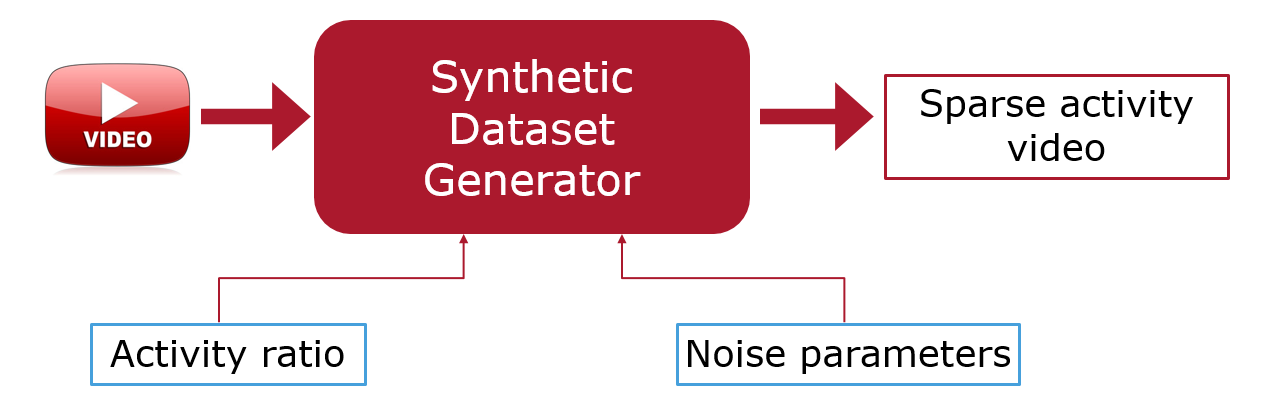
\includegraphics[width=\linewidth]{images/synthetic-dataset-generator.PNG}
    \caption{Synthetic dataset generator}
    \label{fig:synthetic-dataset-generator}
\end{figure}

In order to generate the synthetic data, we follow the following steps:
\begin{enumerate} 
    \item identify background frame
    \item make background block
    \item write background block(s)
    \item write activity block
    \item repeat (3) and (4)
\end{enumerate}

Step 1 is simple. We manually scroll through a video and identify a frame with no activity (ideally no person). In step 2, we repeat the frame $\Delta \times fps$ times where $fps$ is the frame-per-second of original video and $\Delta$ is the target length of background block in seconds. Then we alternatively write background block(s) and activity block in turn. An activity block is simply a section of original video. By default, we use $30s$ long activity blocks. Length of background block is also kept at $30s$ by default. Figure \ref{fig:synthetic-video} helps understand the concept of activity block and synthetic video.  

\begin{figure}
    \centering
    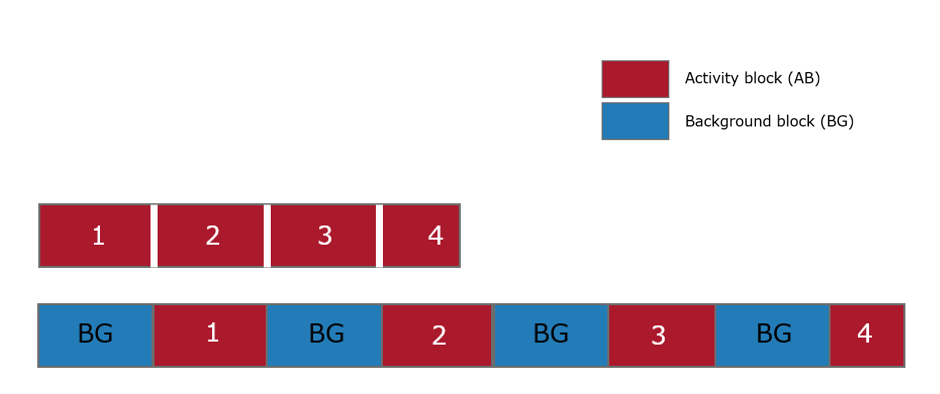
\includegraphics[width=\linewidth]{images/synthetic-video.PNG}
    \caption{Synthetic video illustration}
    \label{fig:synthetic-video}
\end{figure}

An important concept associated with this procedure is \textit{Activity Ratio}. It is defined as 
$$ \text{Activity Ratio} = \text{AR} = \frac{1}{1+nBG} $$
where $nBG=$ number of background blocks per activity block. Figure \ref{fig:synthetic-video} has $nBG=1$. Table \ref{table:activity-ratio} explains the relationship between $nBG$ and AR. 


\begin{table}
\centering
\caption{Relationship of number of background blocks and activity ratio} \vspace{5pt}
\label{table:activity-ratio}
\begin{tabular}{@{}| l | l | l | @{}} \hline
nBG & nAB:nBG & AR   \\ \hline \hline
1   & 1:1     & 0.5  \\
3   & 1:3     & 0.25 \\
5   & 1:5     & 0.16 \\ \hline
\end{tabular}
\end{table}

\subsubsection{Adding noise}
In order to test the robustness of our approach, we also add noise to our synthetic data. Table \ref{table:noise-params} discuses the parameters that control the level of noise. We use \textbf{salt and pepper} noise in our experiments.

In order to add noise, we first select $p\%$ of frames from each background block. Each of the frame is equally likely to be selected. Now we draw an integer $r$ from normal distribution with parameters $\mu$ and $\sigma$. Now for each selected frame, we select $r$ pixels and add noise to them. Again all pixels are equally likely. 

\begin{table}
\centering
\caption{Noise parameters}  \vspace{5pt}
\label{table:noise-params}
\begin{tabular}{|l|l|}
\hline
params & description                              \\ \hline \hline
$p$          & percentage of noisy frames in BG block  \\ 
$\mu$        & avg. no. of noisy pixels in noisy frame     \\ 
$\sigma$     & standard deviation of no. of noisy pixels     \\ \hline
\end{tabular}
\end{table}
